\chapter{Implementation}
\section{Software architecture}
Continue the IMP tool, all the functions for this task was saved in the \textbf{impls\_2015} package of program. Besides the method was created by myself, I also use some methods from the OpenCV (library for image processing) and Qt framework (framework for C++).\\[0.2cm]
\begin{figure}[h!]
\centering
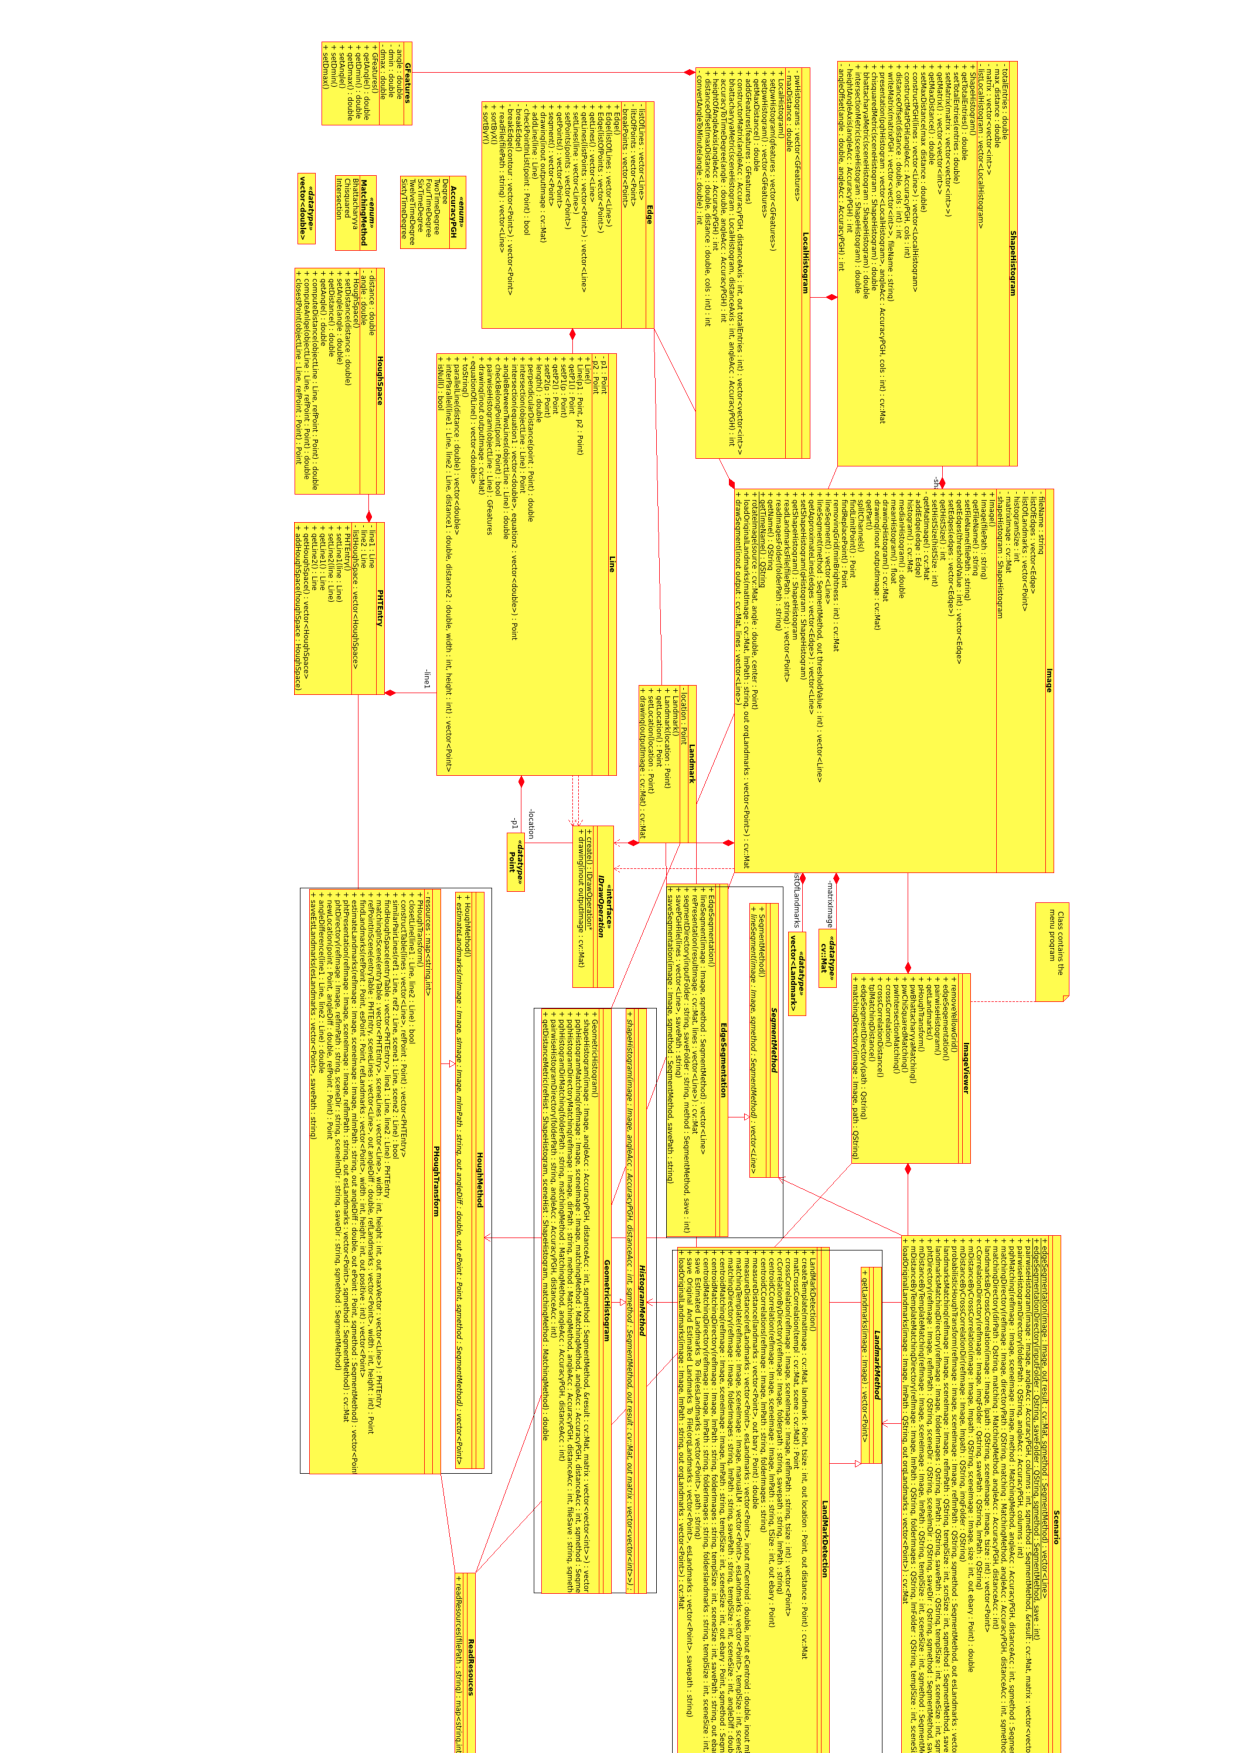
\includegraphics[width=0.9\textwidth]{images/cdiagram}
\caption{The class diagram of program}
\label{fig:cdiagram}
\end{figure}
The class diagram\footnote{See the full image in Appendix} in \ref{fig:cdiagram} show mainly classes of my task. The \textit{mainly} methods located in the \textit{ImageViewer} class, where contains all functions of the software. To represent the information of image and preprocessing about clear the yellow grid, we use the classes such as \textit{Line}, \textit{Edge}, \textit{Landmark}, \textit{YellowGird}, \textit{Image} class. For the edge segmentation, construct the geometric histogram and landmarks detection, we have \textit{GFeatures}, \textit{LocalHistogram}, \textit{ShapeHistogram}, \textit{EdgeSegmentation}, \textit{LandmarkDection} class. All the main functions were inherated from the \textit{IExtraction} interface and used in \textit{main} class via the \textit{Sceneario} class. The aim, properties and methods in each class was discussed in below sections.
\section{Image preprocessing}
The \textit{Image processing} section contains the information about the classes which describe the geometric objects can be represent the image and the method to remove the yellow grid on the images.
\subsection{Line class}
\textbf{Line} class describe the information of a straight line and the methods can do with a line.
\subsubsection{The attributes}
\begin{itemize}
\item\textbf{p1}: the first endpoint of line.
\item\textbf{p2}: the second endpoint of line.
\end{itemize}
\subsubsection{The methods}
\begin{itemize}
\item\textbf{Line()}: Constructor an empty line.
\item\textbf{Line(p1: Point, p2: Point)}: Constructor a line with two endpoints p1, p2. With type of the endpoints is \textbf{Point} (in OpenCV)
\item\textbf{getP1()}: Getter the first endpoint 
\item\textbf{setP1(p:Point)}: Setter the first endpoint
\item\textbf{getP2()}: Getter the second endpoint 
\item\textbf{setP2(p:Point)}: Setter the second endpoint
\item\textbf{length()}: Calculate the length of line
\item\textbf{perpendicularDistance(point:Point)}: Compute the perpendicular distance from point ``\textbf{point}" to the line
\item\textbf{angleBetweenTwoLines(objectLine: Line}: Compute the angle between two lines.
\item\textbf{checkBelongPoint(point: Point)}: Check a point stay on the line or not. If the point stay on the line, the return value is true; otherwise, return false.
\item\textbf{intersection(objectLine: Line)}: Finding the intersection point of two lines. If two lines have intersect, the method will return the coordinate of intersection point; otherwise, method will return a negative point.
\item\textbf{pairwiseHistogram(objectLine: Line)}: Finding the geometric features between two lines. The return value is an \textbf{GFeatures} object, it includes the information of angle between two lines, the distance from two endpoints of \textit{objectLine} to the reference line.
\item\textbf{equationOfLine()}: Calculate the equation of line. 
\item\textbf{drawing(cv::Mat outputImage)}: Drawing the line on the output image.
\end{itemize}
\subsection{Edge class}
\subsection{Image class}
\section{Automatic classification }
about methods
\section{Result}
result...





























